Esta es la línea temporal de la vida de dionisio:

\begin{center}
  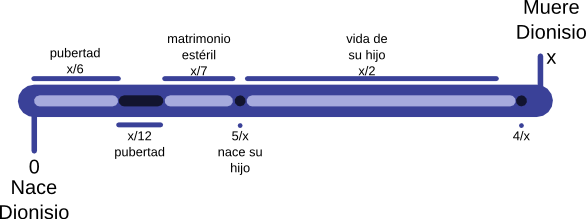
\includegraphics[width=0.9\textwidth]{img/dionisio-lifetime.png}
\end{center}

Se trata de un juego de proporciones, en el que la siguiente ecuación se tiene que cumplir.

\begin{equation*}
  \frac{1}{6} + \frac{1}{12} + \frac{1}{7} + \frac{5}{x} + \frac{1}{2} + \frac{4}{x} = 1
\end{equation*}

Donde $x$ es la edad de Dionisio. Despejando la ecuación, sabremos cuánto vivió Dionisio:

\begin{align*}
  \frac{5+4}{x} &= \frac{3}{28} \\
  x &= 84
\end{align*}
